\documentclass[tikz,border=5pt]{standalone}
\usepackage[T1]{fontenc}
\usepackage{lmodern,amsmath,amssymb}
\usetikzlibrary{arrows.meta,calc,positioning,fit,backgrounds,shapes.geometric,matrix,decorations.pathreplacing,patterns}
\definecolor{ink}{gray}{0.08}
\definecolor{wash}{gray}{0.965}
\definecolor{soft}{gray}{0.45}
\tikzset{box/.style={draw=ink,line width=.65pt,fill=white,align=center,inner sep=4pt,outer sep=0pt,font=\small},flow/.style={draw=ink,line width=.65pt,-{Latex[length=1.8mm,width=1.3mm]},rounded corners=2pt},annotation/.style={font=\scriptsize,text=soft,align=center},groupbox/.style={draw=soft,dashed,line width=.45pt,fill=wash}}
\begin{document}
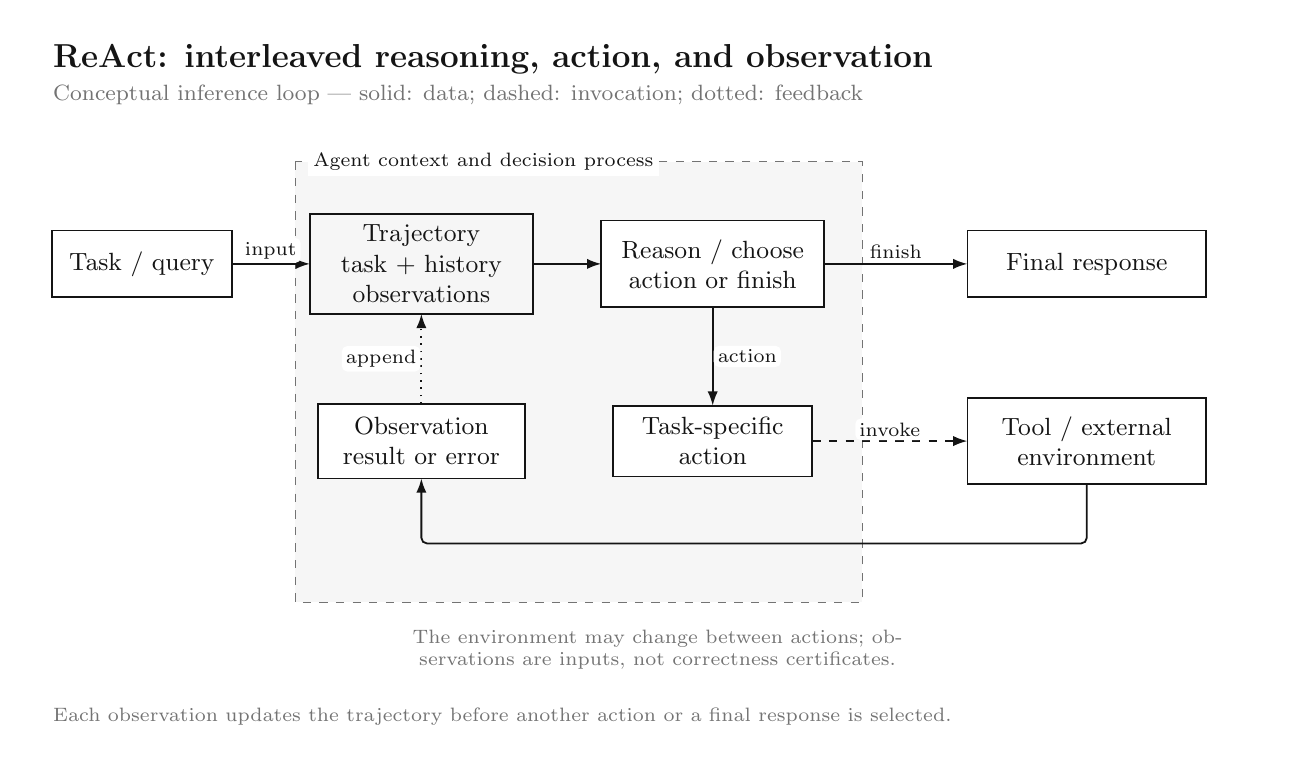
\begin{tikzpicture}[x=1cm,y=-1cm,font=\rmfamily,text=ink]

\path[use as bounding box] (0,0) rectangle (16,9);
\node[anchor=west,font=\large\bfseries] at (.2,.4) {ReAct: interleaved reasoning, action, and observation};
\node[anchor=west,font=\footnotesize,text=soft] at (.2,.85) {Conceptual inference loop | solid: data; dashed: invocation; dotted: feedback};
\begin{pgfonlayer}{background}
\draw[groupbox] (3.4,1.7) rectangle (10.6,7.3);
\node[anchor=west,font=\scriptsize,fill=white,inner sep=2pt] at (3.55,1.7) {Agent context and decision process};
\end{pgfonlayer}
\node[box,minimum width=2.25cm,minimum height=0.85cm,text width=2.0cm] (request) at (1.45,3.0) {Task / query};
\node[box,fill=wash,minimum width=2.8cm,minimum height=1.25cm,text width=2.55cm] (context) at (5.0,3.0) {Trajectory\\task + history\\observations};
\node[box,minimum width=2.8cm,minimum height=1.1cm,text width=2.55cm] (policy) at (8.7,3.0) {Reason / choose\\action or finish};
\node[box,minimum width=2.5cm,minimum height=0.9cm,text width=2.25cm] (call) at (8.7,5.25) {Task-specific\\action};
\node[box,minimum width=2.6cm,minimum height=0.95cm,text width=2.35cm] (observe) at (5.0,5.25) {Observation\\result or error};
\node[box,minimum width=3.0cm,minimum height=1.1cm,text width=2.75cm] (world) at (13.45,5.25) {Tool / external\\environment};
\node[box,minimum width=3.0cm,minimum height=0.85cm,text width=2.75cm] (answer) at (13.45,3.0) {Final response};
\begin{pgfonlayer}{background}
\draw[flow] (request.east) -- (context.west) node[midway,above,fill=white,inner sep=1.5pt,font=\scriptsize] {input};
\draw[flow] (context.east) -- (policy.west);
\draw[flow] (policy.east) -- (answer.west) node[midway,above,fill=white,inner sep=1.5pt,font=\scriptsize] {finish};
\draw[flow] (policy.south) -- (call.north) node[midway,right,fill=white,inner sep=1.5pt,font=\scriptsize] {action};
\draw[flow,dashed] (call.east) -- (world.west) node[midway,above,fill=white,inner sep=1.5pt,font=\scriptsize] {invoke};
\draw[flow] (world.south) -- (13.45,6.55) -- (5.0,6.55) -- (observe.south);
\draw[flow,dotted] (observe.north) -- (context.south) node[midway,left,fill=white,inner sep=1.5pt,font=\scriptsize] {append};
\end{pgfonlayer}
\node[annotation,anchor=center,text width=12cm] at (8.0,7.9) {The environment may change between actions; observations are inputs, not correctness certificates.};
\node[anchor=west,align=left,font=\scriptsize,text=soft,text width=15.6cm] at (.2,8.75) {Each observation updates the trajectory before another action or a final response is selected.};
\end{tikzpicture}
\end{document}
